%!TEX ROOT=../dissertation.tex

\chapter{AVeriTeC Paper}
\section{Introduction}
\label{sec:introduction}
We release \review{a} pipeline for fact-checking claims using evidence retrieved from the web consisting of two modules -- a \textit{retriever}, which picks the most relevant sources among the available knowledge store\footnote{Due to the pre-retrieval step that was used to generate knowledge stores, our \say{retriever} module could more conventionally be referred to as a \say{reranker}, which we refrain from, to avoid confusion with reranking steps it uses as a subroutine.} and an \textit{evidence \& label generator} which generates evidence for the claim using these sources, as well as its veracity label. 

Our pipeline is a variant of the popular Retrieval-augmented Generation (RAG) scheme~\cite{rag}, making it easy to re-implement using established frameworks such as Langchain, Haystack, or our attached Python codebase for future research or to use as a baseline.

This paper describes our pipeline and the decisions taken at each module, achieving a simple yet efficient RAG scheme that improves dramatically across the board over the baseline system from~\cite{averitec2024}, and scores third in the \averitec{} leaderboard as of August 2024, with an \averitec{} test set score of 50.4\%.

% show figures/pipeline.png
\begin{figure}[h]
    \centering
    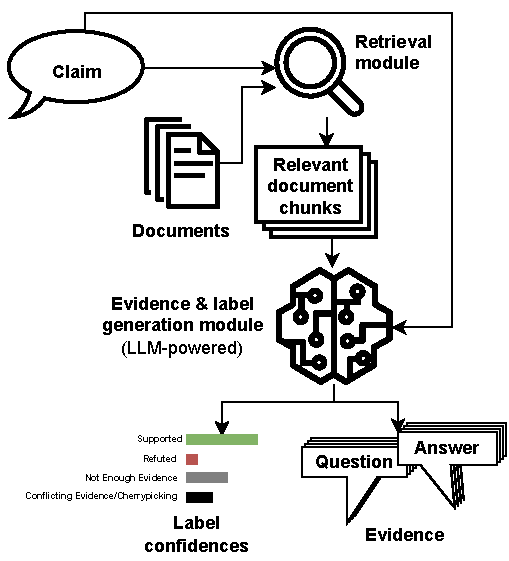
\includegraphics[width=0.47\textwidth]{figures/pipeline.pdf}
    \caption{Our pipeline}
    \label{fig:pipeline}
\end{figure}

\section{Related work}
\label{sec:relwork}
\label{avscore}
\begin{enumerate}
    \item \textbf{\averitec{} shared task}~\cite{averitec2024} releases the datase of real-world fact-checked claims, annotated with evidence available at the date the claim was made.
    
    \review{It proposes the \textbf{\averitec{} Score} -- a method of unsupervised scoring of fact-checking pipeline against this gold data using Hungarian METEOR score, matching the evidence questions (Q) or the whole evidence (Q+A).
    The score is then calculated as the proportion of claims with accurate label and sound evidence (using a threshold for Hu-METEOR such as 0.25) among all claims in the dataset, giving an estimate on \say{how often the whole fact-checking pipeline succeeds end to end}.}

    The provided \textbf{baseline} is a pipeline of search query generation, API search (producing a knowledge store), sentence retrieval, Question-and-answer (QA) generation, QA reranking, QA-wise claim classification and label aggregation, achieving an overall \averitec{} test set score of 11\%.  
    \item \review{\textbf{FEVER Shared Task}~\cite{thorne-etal-2018-fact}, a predecessor to the \averitec{}, worked with a similar dataset engineered on top of the enclosed domain Wikipedic data rather than real-world fact-checks. 
    Its top-ranking solutions used a simpler pipeline of Document Retrieval, Sentence Reranking and Natural Language Inference, improving its modules in a decoupled manner and scoring well above 60\% in a similarly computed FEVER score~\cite{thorne-etal-2018-fever} on this data.}
    \item \textbf{Our previous research} on fact-checking pipelines~\cite{Ullrich2023,drchal2023pipelinedatasetgenerationautomated} using data similar to FEVER and \averitec{} shows significant superiority of fact-checking pipelines that \textbf{retrieve the whole documents} for the inference step, rather than retrieving out-of-context sentences.
    \item \textbf{Retrieval-Augmented Generation (RAG) for Knowledge-Intensive Tasks}~\cite{rag} takes this a step further, leveraging Large Language Model (LLM) for the task, providing it the whole text of retrieved documents (each a chunk of Wikipedia) and simply instructing it to predict the evidence and label on top of it, achieving results within 4.3\% from the FEVER state of the art by the time of its publication (December 2020) \textit{without} engineering a custom pipeline for the task.
\end{enumerate}


\section{System description}
\label{sec:system}
\review{Our system design prioritizes simplicity, and its core idea is using a straightforward RAG pipeline without engineering extra steps, customizing only the retrieval step and LLM prompting } (Listing~\ref{lst:llm_system_prompt} \review{in Appendix~\ref{appendix_sec:system_prompt}}).
Despite that, this section describes and justifies our decisions taken at each step, our additions to the naive version of RAG modules to tune them for the specific task of fact-checking, and their impact on the system performance.

\subsection{Retrieval module}
\label{retrieval}
To ease comparison with the baseline and other systems designed for the task, our system does not use direct internet/search-engine access for its retrieval, but an \averitec{} \textit{knowledge store} provided alongside each claim.

\review{To use our pipeline in the wild, our retrieval module is decoupled from the rest of the pipeline and can be swapped out in favour of an internet search module such as SerpApi\footnote{\url{https://serpapi.com/}} as a whole, or it can be used on top of a knowledge store emulated using large crawled corpora such as CommonCrawl\footnote{\url{https://commoncrawl.org/}} and a pre-retrieval module.}

\subsubsection{Knowledge stores}
Each claim's knowledge store contains pre-scraped results for various search queries that can be derived from the claim using human annotation or generative models.
The knowledge stores used with ours as well as the baseline system can be downloaded from the \averitec{}  dataset page\footnote{\url{https://fever.ai/dataset/averitec.html}}, containing about 1000 pre-scraped \textit{documents}\footnote{\label{devsetnote}The numbers are orientational and were computed on knowledge stores provided for the \averitec{}  dev set.}, each consisting of $28$ sentences at median\footnoteref{devsetnote}, albeit varying wildly between documents.
The methods used for generating the knowledge stores are explained in more detail by~\citet{averitec2024}.
%To use our system in the wild, this knowledge store can be emulated using a search API such as SerpApi, or even a large document collection such as Common Crawl pruned down to similar orders of magnitude using a cheap retrieval method and the claim as a search query.

Our retrieval module then focuses on picking a set of $k$ ($k=10$ in the examples below, as well as in our submitted system) most appropriate document chunks to fact-check the provided claim within this knowledge store.

\subsubsection{Angle-optimized embedding search}
\label{sec:knn}
Despite each article in any knowledge store only needing to be compared \textit{once} with its \textit{one specific} claim, which should be the use-case for CrossEncoder reranking~\cite{dejean2024thoroughcomparisoncrossencodersllms}, our empirical preliminary experiments made us favour a \textit{cosine-similarity} search based on vector embeddings instead.
It takes less time to embed the whole knowledge store into vectors than to match each document against a claim using crossencoder, and the produced embeddings can be re-used across experiments.

For our proof of concept, we explore the MTEB~\cite{muennighoff-etal-2023-mteb} benchmark leaderboard, looking for a reasonably-sized open-source embedding model, ultimately picking Mixedbread's mxbai-large-v1~\cite{li-li-2024-aoe,emb2024mxbai} optimized for the cosine objective fitting our inteded use.

\review{To reduce querying time at a reasonable exactness tradeoff, we use Faiss index~\cite{douze2024faiss,johnson2019billion} to store our vectors, allowing us to only precompute semantical representation once, making the retriever respond rapidly in empirical experiments, allowing a very agile prototyping of novel methods to be used.}
\
\subsubsection{Chunking with added context}
Our initial experiments with the whole \averitec{}  documents for the Document Retrieval step have revealed a significant weakness -- while most documents fit within the input size of the embedding model, outliers are common, often with \textit{hundreds of thousands} characters, exceeding the 512 input tokens with little to no coverage of their content.

Upon further examination, these are typically PDF documents of legislature, documentation and communication transcription -- highly relevant sources real fact-checker would scroll through to find the relevant part to refer. 

This workflow inspires the use of \textit{document chunk retrieval} as used in~\cite{rag}, commonly paired with RAG.
We partition each document into sets of its sentences of combined length of $N$ characters at most.
To take advantage of the full input size of the vector embedding model we use for semantical search, we \review{arbitrarily} set our bound $N=512*4=2048$, \review{where 512 is} the input dimension of common embedding models, 4 often being used as a rule-of-thumb number of characters per token for US English in modern tokenizers~\cite{tokens}.

Importantly, each chunk is  assigned metadata -- the source URL, as well as the full text of the next and previous chunk within the same document.
This way, chunks can be presented to the LLM along with their original context in the generation module, where the length constraint is much less of an issue than in vector embedding.
As shown in~\cite{drchal2023pipelinedatasetgenerationautomated}, fact-checking models benefit from being exposed to larger pieces of text such as paragraphs or entire documents rather than out-of-context sentences.
Splitting our data into the maximum chunks that fit our retrieval model and providing them with additional context may help down the line, preventing the RAG sources from being semantically incomplete.

\subsubsection{Pruning the chunks}
While the chunking of long articles prevents their information from getting lost to retriever, it makes its search domain too large to embed on demand.
As each of the thousands of claims has its own knowledge store, each of possibly tens of thousands of chunks, we seek to omit the chunks having little to no common tokens with our claim using an efficient BM25~\cite{bm25} search for the nearest $\omega$ chunks, setting the $\omega$ to 6000 for dev and 2000 for test claims. 
This yields a reasonably-sized document store for embedding each chunk into a vector, taking an average of 40 s to compute and store using the method described in Section~\ref{sec:knn} for each dev-claim using our Tesla V100 GPU.

This allows a quick and agile production of vectorstores for further querying and experimentation, motivated by the \averitec{}  test data being published just several days before the announced submission deadline.
\review{The pruning also keeps the resource intensity moderate for real-world applications.
However, if time is not of the essence, the step can be omitted.}

\subsubsection{Diversifying sources: MMR}
\review{Our choice of embedding search based on the entire claim rather than generating \say{search queries} introduces less noise and captures the semantics of the whole claim.
It is, however, prone to redundancy among search results, which we address using a reranking by the results' Maximal Marginal Relevance (MMR)~\cite{carbonell-mmr}, a metric popular for the RAG task, which maximizes the search results' score computed as (for $D_i\in P$)
$$\lambda \cdot \mathrm{Sim}(D_i, Q) - (1-\lambda) \cdot \max_{D_j \in S} \mathrm{Sim}(D_i, D_j)$$
$Sim$ denoting the cosine-similarity between embeddings, $Q$ being the search query, and $P$ the pre-fetched set of documents (by a search which simply maximizes their $Sim$ to $Q$), forming $S$ as the final search result, by adding each $D_i$ as MMR-argmax one by one, until reaching its desired size.}

In our system, we set $\lambda=0.75$ to favour relevancy rather than diversity, $|S|=10$ and $|P| = 40$, obtaining a set of diverse sources relevant to each claim at a fraction of cost and complexity of a query-generation driven retrieval, such as that used in~\cite{averitec2024}.

\subsection{Evidence \& label generator}
\label{sec:generation}
The second and the last module on our proposed pipeline for automated fact checking is the Evidence \& Label Generator, which receives a claim and $k$ sources (document chunks), and returns $l$ (in our case, $l=10$) question-answer pairs of evidence abstracted from the sources, along with the veracity verdict -- in \averitec{} dataset, a claim may be classified as \textit{Supported}, \textit{Refuted}, \textit{Not Enough Evidence}, or \textit{Conflicting Evidence/Cherrypicking} with respect to its evidence.

Our approach leverages a Large Language Model (LLM), instructing it to output both evidence and the label in a single step, as a chain of thought.
We rely on JSON-structured output generation with source referencing using a numeric identifier, we estimate the label confidences using Likert-scale ratings.
The full system prompt can be examined in Listing~\ref{lst:llm_system_prompt} \review{in Appendix~\ref{appendix_sec:system_prompt},} and this section further explains the choices behind it.

\subsubsection{JSON generation}

To be able to collect LLM's results programmatically, we exploit their capability to produce structured outputs, which is on \review{the} rise, with datasets available for tuning~\cite{tang2024strucbenchlargelanguagemodels} and by the time of writing of this paper (August 2024), systems for strictly structured prediction are beginning to be launched by major providers~\cite{json}.

Despite not having access to such structured-prediction API by the time of \averitec{} shared task, the current generation of models examined for the task (section~\ref{sec:chosen_llms}) rarely strays from the desired format if properly explained within a system prompt -- we instruct our models to output a JSON of pre-defined properties (see prompt Listing~\ref{lst:llm_system_prompt} \review{in Appendix~\ref{appendix_sec:system_prompt}}) featuring both evidence and the veracity verdict for a given claims.

Although we implement fallbacks, less than 0.5\% of our predictions \review{threw} a parsing exception throughout experimentation, and could be easily recovered using the same prompting again, exploiting the intrinsic randomness of LLM predictions.

\subsubsection{Chain-of-thought prompting}
While JSON dictionary should be order-invariant, we can actually exploit the order of outputs in our output structure to make LLMS like GPT-4o output better results~\cite{cot}.
This is commonly referred to as the \say{chain-of-thought} prompting -- if we instruct the autoregressive LLM to first output the evidence (question, then answer), then a set of all labels with their confidence ratings (see section~\ref{likert}) and only then the final verdict, its prediction is both cheaper as opposed to implementing an extra module, as well as more reliable, as it must attend to all of the intermediate steps as well.

\subsubsection{Source referring}
To be able to backtrack the generated evidence to the urls of the used sources, we simply augment each question-answer pair with a source field.
We assign a 1-based index\footnote{\review{We chose the 1-based source indexing to exploit the source-referring data in LLM train set such as Wikipedia, where source numbers start with 1. The improvement in quality over 0-based indexing was not experimentally tested.}}  to each of the sources to facilitate tokenization and prompt the LLM to refer it as the source ID with each evidence it generates.
While hallucination can not be fully prevented, it is less common than it may appear -- with RAG gaining popularity, the models are being trained to cite their sources using special citation tokens~\cite{menick2022teachinglanguagemodelssupport}, not dissimilarly to our proposal.

\subsubsection{Dynamic few-shot learning}
To utilise the few-shot learning framework~\cite{fewshot} shown to increase quality of model output, we provide our LLMs with examples of what we expect the model to do.
To obtain such examples, our evidence generator looks up the \averitec{} train set using BM25 to get the 10 most similar claims, providing them as the few-shot examples, along their gold evidence and veracity verdicts.
Experimentally, we also few-shot our models to output an \textit{answer type} (\textit{Extractive}, \textit{Abstractive}, \textit{Boolean},\dots) as the \textit{answer type} is listed with each sample anyways, and we have observed its integration into the generation task to slightly boost our model performance.

\subsubsection{Likert-scale label confidences}
\label{likert}
Despite modern LLMs being well capable of predicting the label in a \say{pick one} fashion, research applications such as ours may prefer them to output a probability distribution over all labels for two reasons.

Firstly, it measures the confidence in each label, pinpointing the edge-cases, secondly, it allows ensembling the LLM classification with any other model, such as Encoders with classification head finetuned on the task of Natural Language Inference (NLI) (see section~\ref{subsubsec:ensembling}).

As the LLMs and other token prediction schemes struggle with the prediction of continuous numbers which are notoriously hard to tokenize appropriately~\cite{golkar2023xvalcontinuousnumberencoding}, we come up with a simple alternative: instructing the model to print each of the 4 possible labels, along with their Likert-scale rating: 1 for \say{strongly disagree}, 2 for \say{disagree}, 3 for \say{neutral}, 4 for \say{agree} and 5 for \say{strongly agree}~\cite{likert1932technique}.

On top of the ease of tokenization, Likert scale's popularity in psychology and other fields such as software testing~\cite{likertstudy} adds another benefit -- both the scale itself and its appropriate usage were likely demonstrated many times to LLMs during their unsupervised training phase.

To convert the ratings such as \texttt{\{\say{Supported}:2, \say{Refuted}:5, \say{Cherrypicking}:4, \say{NEE}:2\}} to a probability distribution, we simply use softmax~\cite{NIPS1989_0336dcba}.
While the label probabilities are only emulated (and may only take a limited, discrete set of values) and the system may produce ties, it gets the job done until further research is carried out.

\subsubsection{Choosing LLM}
\label{sec:chosen_llms}
In our experiments, we have tested the full set of techniques introduced in this section, computing the text completion requests with:
\begin{enumerate}
    \item GPT-4o (version \texttt{2024-05-13})
    \item Claude-3.5-Sonnet (\texttt{2024-06-20}), using the Google's Vertex API
    \item LLaMA 3.1 70B, in the final experimets to see if the pipeline can be re-produced using open-source models
\end{enumerate} 

Their comparison can be seen in tables~\ref{tab:nli} and~\ref{tab:pipeline_scores}; for our submission in the \averitec{}  shared task, GPT-4o was used.

%!TEX ROOT=../emnlp2023.tex
\section{Other examined approaches}
\label{sec:failed}
In this section, we also describe a third, optional module we call the \textit{veracity classifier}, which takes the claim and its evidence generated by our evidence \& label generator~(section~\ref{sec:generation}) and predicts the veracity label independently, based on the suggested evidence, using a fine-tuned NLI model.
We also describe the options of its ensembling with veracity labels predicted in the generative step (section~\ref{likert}).

The absence of a dedicated veracity classifier has not been shown to decrease the performance of our pipeline significantly (as shown, e.g., in tables~\ref{tab:pipeline_scores} and~\ref{tab:nli}) so we suggest to omit this step altogether and we proceed to participate in the \averitec{}  shared task without it, proposing a clean and simple RAG pipeline without the extra step (Figure~\ref{fig:pipeline}) for the fact-checking task.

\subsection{Single-evidence classification with label aggregation}
In the earliest stages of experimenting, we utilized the baseline classifier provided by \averitec{} authors\footnote{\url{https://huggingface.co/chenxwh/AVeriTeC}}~\cite{averitec2024}.
It is based on the BERT~\cite{devlin-etal-2019-bert} and was further fine-tuned on the \averitec{}  dataset~\cite{averitec2024}. 
It takes one claim and one question-answer evidence as input -- each claim therefore has multiple classifications, one for each evidence. The classifications are then aggregated using a heuristic of several if-clauses to determine the final label. 

We experiment with altering this heuristic (e.g. by making \textit{not enough evidence} the final label only when no other labels are present at any evidence), and training NLI models that could work better with it, such as 3-way DeBERTaV3~\cite{he2023debertav3improvingdebertausing} without a breakthrough result, motivating a radically different approach.

\subsection{Multi-evidence classification}
\label{subsubsec:concatenation}
The multi-evidence approach is to fine-tune a 4-way Natural Language Inference (NLI) classifier, using the full scope of evidence directly at once, without heuristics.
For that, we concatenate all of the evidence together using a separator \texttt{[SEP]} token. This allows the model to know exact question-answer borders, albeit using a space has turned out to be just as accurate as the experiments went on. As the veracity verdict should be independent of the evidence ordering, we also experiment with sampling different permutations in the fine-tuning step to increase the size of our data.

We carry out the fine-tuning using the \averitec{} train split with gold evidence and labels on \mbox{DeBERTaV3}~\cite{he2023debertav3improvingdebertausing} in two variants: the original large one\footnote{\url{https://huggingface.co/microsoft/deberta-v3-large}} and one pre-finetuned on NLI tasks\footnote{\url{https://huggingface.co/cross-encoder/nli-deberta-v3-large}}, and also Mistral-7B-v0.3 model\footnote{\url{https://huggingface.co/mistralai/Mistral-7B-v0.3}} with a classification head (MistralForSequenceClassification) provided by the Huggingface Transformers library~\cite{wolf-etal-2020-transformers} that utilizes the last token. In the preliminary testing phase, the original DeBERTaV3 Large performed the best and was used in all other experimental settings.

From the approaches described above, we achieved the best results for the development split with gold evidence and labels with a model without permuting the evidence, achieving 0.71 macro $F_1$ score using a space-separation. The \texttt{[SEP]} model achieved a comparable 0.70 macro $F_1$ score, and the random order model performed worse with a 0.67 macro $F_1$ score, all improving significantly upon baseline, yet falling behind the capabilities of generating the labels alongside evidence in a single chain-of-thought. 
We provide our best DeBERTaV3 finetuned model publicly in a Huggingface repository\footnote{\url{https://huggingface.co/ctu-aic/deberta-v3-large-AVeriTeC-nli}}.

\subsection{Ensembling classifiers}
\label{subsubsec:ensembling}

Encouraged by the promising results of our multi-evidence classifiers, we go on to try to ensemble the models with LLM predictions from section~\ref{likert}, using a weighted average of the class probabilities of our models.
We have experimented with multiple weight settings: 0.5:0.5 for even votes, 0.3:0.7 in favour of the LLM to exploit its accuracy while tipping its scales in cases of a more spread-out label probability distribution, as well as 0.1:0.9 to use the fine-tuned classifier only for tie-breaking, listing the results in Table~\ref{tab:nli}.

We also tried tuning our ensemble weights based on a subset of the dev split, without a breakthrough in accuracy on the rest of dev samples.

The last method we tried was stacking using logistic regression. However, this setup classified no labels from \textit{Not Enough Evidence} and \textit{Conflicting Evidence/Cherrypicking}, and we could not achieve reasonable results. For logistic regression, we used the scikit-learn library~\cite{scikit-learn}.

We conclude that the augmentation of the pipeline from Figure~\ref{fig:pipeline} with a classification module using a single NLI model or an ensemble with LLM is unneccessary, as it adds complexity and computational cost without paying off on the full pipeline performance (Table~\ref{tab:pipeline_scores}).

\subsection{Conflicting Evidence/Cherrypicking detection}

During the experiments, we discovered that classifying the \textit{Conflicting Evidence/Cherrypicking} class is the most challenging task, achieving a near-zero $F_1$-score across our various prototype pipelines.
To overcome this problem, we tried to build a binary classifier with cherrypicking as positive class. We tried to use the DeBERTaV3 Large model with both basic and weighted cross-entropy loss (other experimental settings were the same as in section~\ref{subsubsec:concatenation}), but it could not pick up the training task due to the \textit{Conflicting Evidence/Cherrypicking} underrepresentation in train set -- less than 7\% of the samples carry the label. 

Even after exploring various other methods, we did not get a reliable detection scheme for this task, perhaps motivating a future collection of data that represents the class better.
While writing this system description paper, we found an interesting research by~\citet{jaradat2024contextawaredetectioncherrypickingnews} that uses a radically different approach to detect cherrypicking in newspaper articles.


\section{Results and analysis}
\label{sec:results}

We examine our pipeline results using two sets of metrics -- firstly, we measure the prediction accuracy and $F_1$ over predict labels without any ablation, that is obtaining predicted labels using the predicted evidence generated on top the predicted retrieval results. 
While the retrieval module is fixed throughout the experiment (a full scheme described in section~\ref{retrieval}), various Evidence \& Label generators and classifiers are compared in Table~\ref{tab:nli}, showcasing their performance on the same sources.
The results show that if we disregard the quality of evidence, models are more or less interchangeable, without a clear winner across the board -- an ensemble of DeBERTA and Claude-3.5-Sonnet gives the best $F_1$ score, while GPT-4o scores 72\% accuracy.
\begin{table}    \centering
    \setlength\tabcolsep{3pt} % default value: 6pt
    \resizebox{0.6\columnwidth}{!}{%
    \begin{tabular}{lcccc}
        \toprule
        \textbf{Classifier} & \textbf{Acc} & \textbf{$F_1$} & \textbf{Prec.} & \textbf{{\footnotesize {Recall}}} \\
        \midrule
        GPT4o & 0.72 & 0.46 & 0.48 & 0.47 \\
        Claude 3.5 Sonnet & 0.64 & 0.49 & 0.50 & 0.52 \\
        DeBERTa & 0.63 & 0.39 & 0.40 & 0.41 \\
        DeBERTa - random@10 & 0.65 & 0.41 & 0.41 & 0.44 \\
        $0.5\cdot\mbox{DeBERTa}+0.5\cdot\mbox{GPT4o}$ & 0.70 & 0.43 & 0.41 & 0.45 \\
        $0.5\cdot\mbox{DeBERTa}+0.5\cdot\mbox{Claude}$ & 0.68 & 0.47 & 0.50 & 0.49 \\
        $0.3\cdot\mbox{DeBERTa}+0.7\cdot\mbox{GPT4o}$ & 0.72 & 0.45 & 0.45 & 0.46 \\
        $0.3\cdot\mbox{DeBERTa}+0.7\cdot\mbox{Claude}$ & 0.66 & \textbf{0.50} & \textbf{0.51} & \textbf{0.53} \\
        $0.1\cdot\mbox{DeBERTa}+0.9\cdot\mbox{GPT4o}$ & {0.72} & 0.39 & 0.46 & 0.43 \\
        $0.1\cdot\mbox{DeBERTa}+0.9\cdot\mbox{Claude}$ & 0.64 & 0.49 & 0.50 & 0.54 \\
        \midrule
        Llama 3.1 & \textbf{0.73} & 0.44 & 0.43 & 0.46 \\
        \bottomrule
    \end{tabular}
    }
    \caption{Evalution of the label generators, classifier models and their ensembles on the \averitec development set. $F_1$, Precision and Recall are computed as macro-averages. The random@10 suffix indicates that the classifier used average of 10 different random orders of QA pairs for each claim. GPT4o stands for the Likert classifier based on GPT-4o, Claude 3.5 Sonnet is the Likert classifier based on Claude 3.5 Sonnet, and DeBERTa is classifier based on DeBERTaV3 Large fine-tuned on \averitec{} gold evidence and labels.}
    \label{tab:nli}
\end{table}
\begin{table*}    \centering
    \begin{tabular}{l | c c c | c c c}
    \hline
    &\multicolumn{3}{c|}{\textbf{Dev Set Scores}} & \multicolumn{3}{c}{\textbf{Test Set Scores}}  \\
    \textbf{Pipeline Name} & \textbf{Q only} & \textbf{Q+A} & \textbf{\averitec{}} & \textbf{Q only} & \textbf{Q+A} & \textbf{AVeriTeC} \\ \hline
    \textbf{GPT-4o (full-featured pipeline)}      & \textbf{0.46} & \textbf{0.29} & \textbf{0.42} & 0.46 & \textbf{0.32} & \textbf{0.50}\\
    GPT-4o s         & 0.45 & 0.28 & 0.38 & 0.45 & 0.30 & 0.47 \\
    Claude-3.5 f             & 0.43 & 0.28 & 0.35 & 0.42 & 0.30 & 0.46 \\
    GPT-4o de              & 0.45 & 0.28 & 0.36 & -- & -- & --\\
    \averitec{} bl            & 0.24 & 0.19 & 0.09 & 0.24 & 0.20 & 0.11\\
    \hline
    Llama 3.1 70B & \textbf{0.46} & 0.27 & 0.36 & \textbf{0.47} & 0.29 & 0.42\\
    \bottomrule
    \end{tabular}
    \caption{Comparison of Pipeline Scores on Dev and Test Sets. \review{Q, Q+A are Hu-METEOR scores against gold data,} AVeriTeC scores \review{are calculated as referred in section~\ref{avscore} thresholded at 0.25}. \say{Full-featured} pipelines use the all the improvement techniques introduced in section~\ref{sec:system}, while the simplified pipeline omits the dynamic few-shot learning, answer-type-tuning and Likert-scale confidence emulation described in section~\ref{sec:generation}}
    \label{tab:pipeline_scores}\end{table*}

In real world, however, the evidence quality is critical for the fact-checking task.
We therefore proceed to estimate it using the hu-METEOR evidence question score, QA score and \averitec{} score benchmarks briefly explained in Section~\ref{avscore} and in greater detail in~\cite{averitec2024}.
We use the provided \averitec{} scoring script to calculate the values for Table~\ref{tab:pipeline_scores}, using its EvalAI blackbox to obtain the test scores without seeing the gold test data.

The latter experiments shown in Table~\ref{tab:pipeline_scores} suggests the superiority of GPT-4o to predict the results for our pipeline with a margin.
Even if we simplify the evidence \& label generation step by omitting the dynamic few-shot learning (section~\ref{sec:generation}), answer-type tuning and Likert-scale confidence emulation, it still scores above others, also showing that our pipeline can be further simplified when needed.
Regardless of the LLM in use, the results of our pipeline improve upon the \averitec{} baseline dramatically.

Posterior to the original experiments and to the \averitec{} submission deadline, we also compute the pipeline results using an open-source model -- the Llama 3.1 70B\footnote{\url{https://huggingface.co/hugging-quants/Meta-Llama-3.1-70B-Instruct-AWQ-INT4}}~\cite{dubey2024llama3herdmodels} obtaining encouraging scores, signifying our pipeline being adaptable to work well without the need to use a blackboxed proprietary LLM.

\subsection{API costs}
During our experimentation July 2024, we have made around 9000 requests to OpenAI's \texttt{gpt-4o-2024-05-13} batch API, at a total cost of \$363.
This gives a mean cost estimate of \$0.04 per a single fact-check (or \$0.08 using the API without the batch discount) that can be further reduced using cheaper models, such as \texttt{gpt-4o-2024-08-06}.

We argue that such costs make our model suitable for further experiments alongside human fact-checkers\review{,} whose time spent reading through each source and proposing each evidence by themselves would certainly come at a higher price.

Our successive experiments with Llama 3.1~\cite{dubey2024llama3herdmodels} show promising results as well, nearly achieving parity with GPT.
The use of open-source models such as LLaMa or Mistral allows running our pipeline on premise, without leaking data to a third party and billing anything else than the computational resources.
For further experiments, we are looking to integrate them into the attached Python library using VLLM~\cite{vllm}.

\subsection{Error analysis}
In this section, we provide the results of an explorative analysis of 20 randomly selected samples from the development set. We divide our description of the analysis into the pipeline and dataset errors.


\subsubsection{Pipeline errors}
Our pipeline tends to rely on unofficial (often newspaper) sources rather than official government sources, e.g., with a domain ending or containing \texttt{gov}. On the other hand, it seems that the annotators prefer those sources. This could be remedied by implementing a different source selection strategy, preferring those official sources. For an example, see Listing~\ref{lst:gov_error} \review{in Appendix~\ref{appendix_sec:errors}}.

Another thing that could be recognised as an error is that our pipeline usually generates all ten allowed questions (upper bound given by the task~\cite{averitec2024}). The analysis of the samples shows that the last questions are often unrelated or redundant to the claim and do not contribute directly to better veracity evaluation. However, since the classification step of our pipeline is not dependent on the number of question-answer pairs, this is not a critical error.
Listing~\ref{lst:unrelated_questions} \review{in Appendix~\ref{appendix_sec:errors}} shows an example of a \review{data point} with some unrelated questions.

When the pipeline generates extractive answers, it sometimes happens that the answer is not precisely extracted from the source text but slightly modified. An example of this error can be seen in Listing~\ref{lst:extractive_error} \review{in Appendix~\ref{appendix_sec:errors}}. This error is not critical, but it could be improved in future works, e.g. using post-processing via string matching.

Individual errors were also caused by the fact that we do not use the claim date in our pipeline and because our pipeline cannot analyse PDFs with tables properly. The last erroneous behaviour we have noticed is that the majority of questions and answers are often generated from a single source. This should not be viewed as an error, but by introducing diversity into the sources, the pipeline would be more reliable when deployed in real-world scenarios.

\subsubsection{Dataset errors}
During the error analysis of our pipeline, we also found some errors in the \averitec{} dataset that we would like to mention. In some cases, there is a leakage of PolitiFact \review{or Factcheck.org} fact-checking articles where the claim is already fact-checked. This leads to a situation where our pipeline gives a correct verdict using the leaked evidence. However, annotators gave a different label (often Not Enough Evidence). \review{An example of this error is shown in Listing~\ref{lst:polifact_leakage} in Appendix~\ref{appendix_sec:errors}}. 

Another issue we have noticed is the inconsistency in the questions and answers given by annotators. \review{Sometimes, they tend to be longer, including non-relevant information, while some are much shorter, as seen in Listing~\ref{lst:different_lengths} in Appendix~\ref{appendix_sec:errors}}. The questions are often too general, or the annotators seem to use outside knowledge. This inconsistency in the dataset leads to a decreased performance of any models evaluated on this dataset.

\subsubsection{Summary}
Despite the abovementioned errors, the explorative analysis revealed that our pipeline consistently gives reasonable questions and answers for the claims. Most misclassified samples in those 20 data points were due to dataset errors.


\section{Conclusion}
\label{sec:conclusion}
In this paper, we describe the use and development of a RAG pipeline over real world claims and data scraped from the web for the \averitec{} shared task.
Its main advantage are its simplicity, consisting of just two decoupled modules -- Retriever and an Evidence~\& Label Generator -- and leveraging the trainable parameters of a LLM rather than on complex pipeline engineering.
The LLMs capabilities may further improve in future, making the upgrades of our system trivial.

In section~\ref{sec:system}, we describe the process of adding features to both modules well in an iterative fashion, describing real problems we have encountered and the justifications of their solution, hoping to share our experience on how to make such systems robust and well-performing.
We publish our failed approaches in section~\ref{sec:failed} and the metrics we observed to benchmark our systems in section~\ref{sec:results}. 
We release our Python codebase to facilitate further research and applications of our system, either as a baseline for future research, or for experimenting alongside human fact-checkers.

\subsection{Future works}
\begin{enumerate}
    \item Integrating a search API for use in real-world applications
    \item Re-examine the Likert-scale rating (section~\ref{likert}) to establish a more appropriate and fine-grained means of tokenizing the label probabilities
    \item Generating evidence in the form of declarative sentences rather than Question-Answer pairs should be explored to see if it leads for better or worse fact-checking performance
    \item RAG-tuned LLMs such as those introduced in~\cite{menick2022teachinglanguagemodelssupport} could be explored to see if they offer a more reliable source citing
\end{enumerate}